\documentclass[conference, a4paper, 10pt, twocolumn]{IEEEtran}
\usepackage{amsmath,amssymb,amsfonts}
\usepackage{algorithmic}
\usepackage{graphicx}
\usepackage{textcomp}
\usepackage{xcolor}
\usepackage[style=ieee]{biblatex}
\usepackage[nottoc]{tocbibind}
\def\BibTeX{{\rm B\kern-.05em{\sc i\kern-.025em b}\kern-.08em
    T\kern-.1667em\lower.7ex\hbox{E}\kern-.125emX}}

\addbibresource{literature_list.bib}
\renewcommand*{\bibfont}{\small}
\begin{document}

\title{Mechanisms to Raise Awareness about Smartwatch Data Collection}

\author{
	\IEEEauthorblockN{
		Mehmed Mustafa
	}
	\IEEEauthorblockA{
		\textit{Institute of Computer Science}\\
		\textit{University of G\"{o}ttingen}\\
		G\"{o}ttingen, Germany\\
		Email: mehmed.mustafa@stud.uni-goettingen.de
	}
	\and
	\IEEEauthorblockN{
		Chris Warin
	}
	\IEEEauthorblockA{
		\textit{Institute of Computer Science}\\
		\textit{University of G\"{o}ttingen}\\
		G\"{o}ttingen, Germany\\
		Email: chris.warin@stud.uni-goettingen.de
	}
}

\maketitle
\thispagestyle{plain}
\pagestyle{plain}


\begin{abstract}
This document is a model and instructions for \LaTeX.
This and the IEEEtran.cls file define the components of your paper [title, text, heads, etc.]. *CRITICAL: Do Not Use Symbols, Special Characters, Footnotes, 
or Math in Paper Title or Abstract.
\end{abstract}

\begin{IEEEkeywords}
component, formatting, style, styling, insert
\end{IEEEkeywords}

\section{Introduction}
Test \cite{shu2016cardea}
\section{Foundations}

\section{Related Work}

\section{Approach}

\section{Discussion}

\section{Conclusion}


\begin{figure*}[htbp]
\centerline{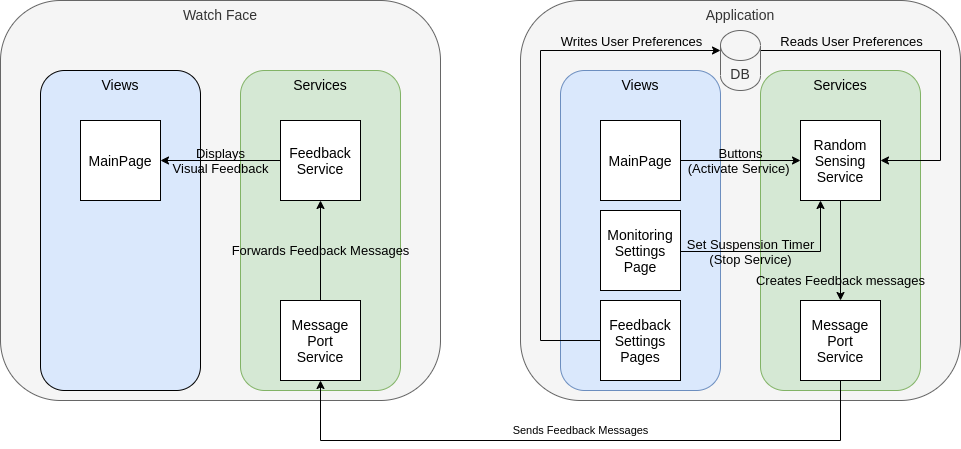
\includegraphics[width=.5\textwidth]{img/appDiagram.png}}
\caption{Example of a figure caption.}
\label{fig}
\end{figure*}

\section*{Acknowledgment}

\printbibliography

\end{document}
